% Dokumentace projektu GAL 2014
% Vendula Poncová, xponco00
% Alena Chernikava, xcerni07

\documentclass[a4paper, 11pt, titlepage, final]{article}[3. prosinec 2011]

\newcommand{\uv}[1]{\quotedblbase #1\textquotedblleft}
\newcommand{\mensi}{$<$}
\newcommand{\vetsi}{$>$}

\usepackage[left=2.5cm,text={16cm, 25cm},top=2cm]{geometry}
\usepackage[czech]{babel}
\usepackage[utf8]{inputenc}
\usepackage[IL2]{fontenc}
\usepackage[dvipdf]{graphicx}
\usepackage{color}

\newcommand{\url}[1]{\textit{#1}}
\begin{document}

%%%%%%%%%%%%%%%%%%%%%%%%%%%%%%%%%%%%%%%%%%%%%%%%%%%%%%%%%%%%%%%%%%%%%%%%%
% titulni strana - DON'T TOUCH! MAGIC!

\begin{titlepage}
\begin{center}

\textsc{
\Large Fakulta informačních technologií 
\medskip\\
Vysoké učení technické v~Brně}

\vspace{\stretch{0.190}}

{\parbox{5cm}{\centering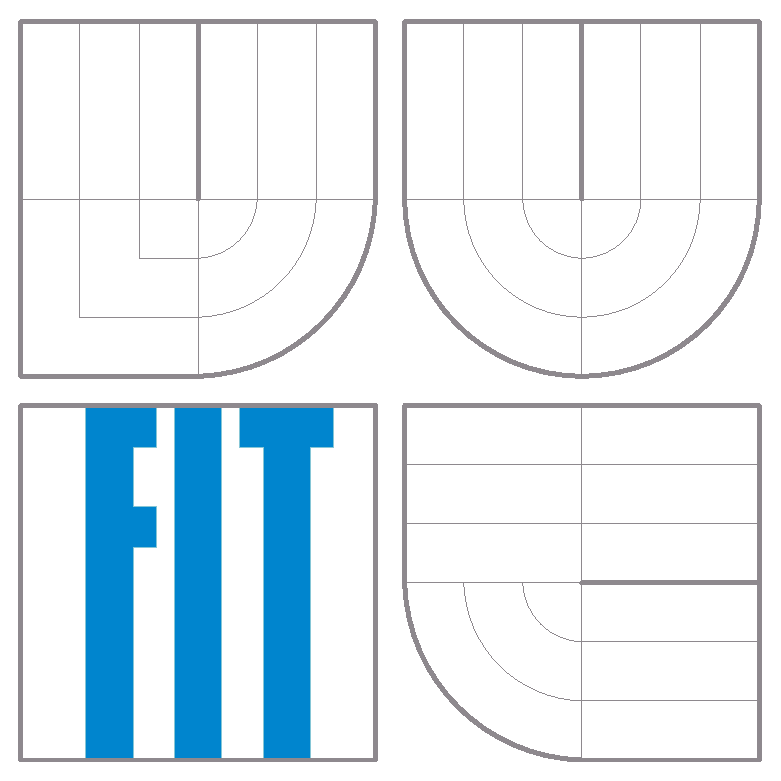
\includegraphics[height=5cm]{img/logo.eps}}}

\vspace{\stretch{0.190}}

{\LARGE Dokumentace projektu do předmětu GAL} \medskip \\
{\Large Paralelizace Egerváryho algoritmu} 


\vspace{\stretch{0.618}}

\end{center}

{\large
Tým 33

Vendula Poncová (\texttt{xponco00})

Alena Chernikava (\texttt{xcerni07})
} \hfill {\large\today}

\end{titlepage}

%%%%%%%%%%%%%%%%%%%%%%%%%%%%%%%%%%%%%%%%%%%%%%%%%%%%%%%%%%%%%%%%%%%%%%%%%
% text dokumentace

\pagenumbering{arabic}
\setcounter{page}{1}

%%%%%%%%%%%%%%%%%%%%%%%%%%%%%%%%%%%%%%%%%%%%%%%%%%%%%%%%%%%%%%%%%%%%%%%%%
\section{Úvod}

%%%%%%%%%%%%%%%%%%%%%%%%%%%%%%%%%%%%%%%%%%%%%%%%%%%%%%%%%%%%%%%%%%%%%%%%%
\section{Egerváryho algoritmus} \label{secEgervary}


\begin{figure}[ht]
  \centering
  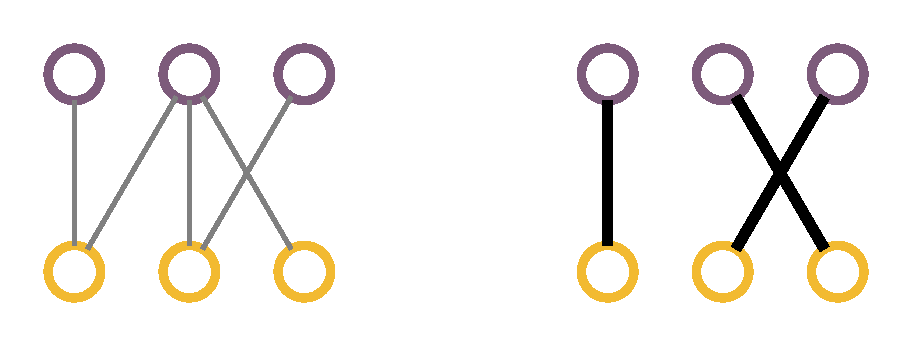
\includegraphics[scale=0.5]{img/bipartite.eps}
  \caption{Bipartitní graf a maximální párování v tomto grafu.}
  \label{imgBipartite}
\end{figure}

\begin{figure}[ht]
  \centering
  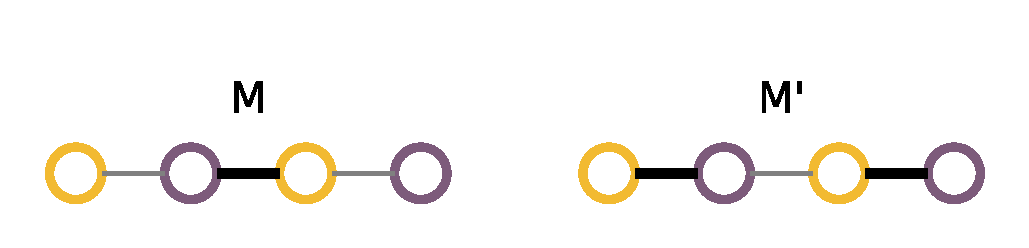
\includegraphics[scale=0.5]{img/mpath.eps}
  \caption{M-rozšiřující cesta a nové párování M'.}
  \label{imgPath}
\end{figure}

\begin{figure}[ht]
  \centering
  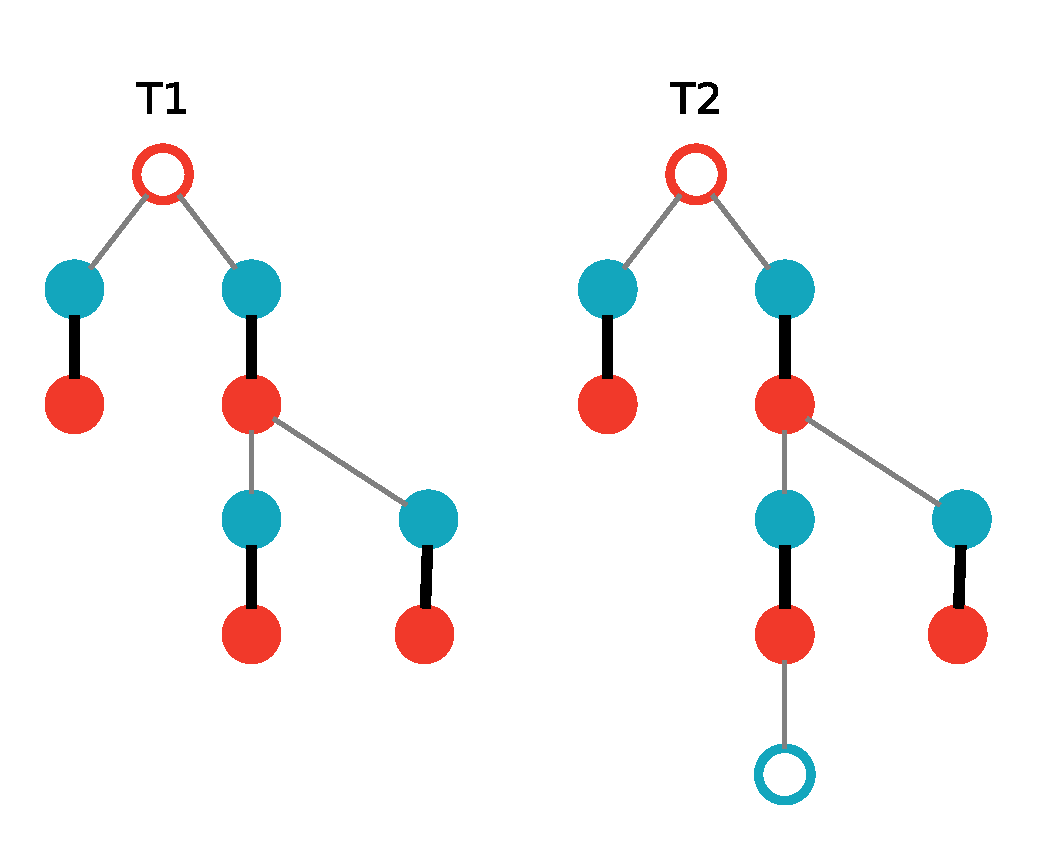
\includegraphics[scale=0.5]{img/trees.eps}
  \caption{M-pokrytý u-strom a M-alternující u-strom.}
  \label{imgTrees}
\end{figure}

%%%%%%%%%%%%%%%%%%%%%%%%%%%%%%%%%%%%%%%%%%%%%%%%%%%%%%%%%%%%%%%%%%%%%%%%%
\section{Sekvenční varianta algoritmu}

\subsection{Návrh řešení}

Vzhledem k tomu, že algoritmus sekvenční varianty je popsán v kapitole \ref{secEgervary}, zbývá vhodně navrhnout datové struktury. 

Algoritmus s grafem pracuje tak, že přechází z uzlu na sousední uzly. Navíc, o hustotě vstupních grafů nic nevíme, proto je vhodnou reprezentací seznam sousedů. Potřebujeme reprezentovat bipartitní neorientovaný graf. Každý hrana tedy bude zastoupena dvakrát, jednou v každém směru. Vhledem k tomu, že atributem hrany je v našem případě příslušnost do párování M, je třeba nějak sdružit odpovídající si hrany. To je možné například tak, že každá hrana bude obsahovat ukazatel na hranu opačnou. Pokud se pak v jedné hraně změní příslušnost do M, lze okamžitě upravit příslušnost opačné hrany.

Uzly se po jednom připojují ke stromu, dokud se nenalezne $M$-rozšiřující cesta, nebo APS tree. Pokud se nalezne cesta, je nutné projít stromem po této cestě a upravit na jejích hranách párování. Proto je výhodné si u každého uzlu pamatovat hranu z jeho předchůdce. Cestu pak lze projít od listového uzlu ke kořeni v lineárním čase k výšce stromu. 

Pokud je nalezen APS tree, je třeba uzly stromu nějak vyloučit z grafu. Stejně tak, po zpracování cesty je třeba uzly stromu uvolnit pro další stromy (říkáme, že strom je zahozen). Pokud bychom uzly zpracovávaly po jednom, bude časová složitost každé takové úpravy stromu linerání vůči počtu uzlů ve stromu. Nabízí se vytvořit datovou strukturu stromu, která bude obsahovat položku se statusem stromu. Uzly stromu se pak budou odkazovat na tuto strukturu. Pokud bude status stromu \texttt{FREE}, pak jsou uzly bílé a dostupné pro nový strom. Pokud je status \texttt{ACTUAL}, uzly jsou modré nebo červené a jsou součástí právě zpracovávaného stromu. Jestliže je status \texttt{APSTREE}, pak jsou uzly zelené a algoritmus je ignoruje. Změna statusu je pak možná v konstatním čase. Příklad takové datové struktury je na obrázku \ref{imgStructure}.

\begin{figure}[ht]
  \centering
  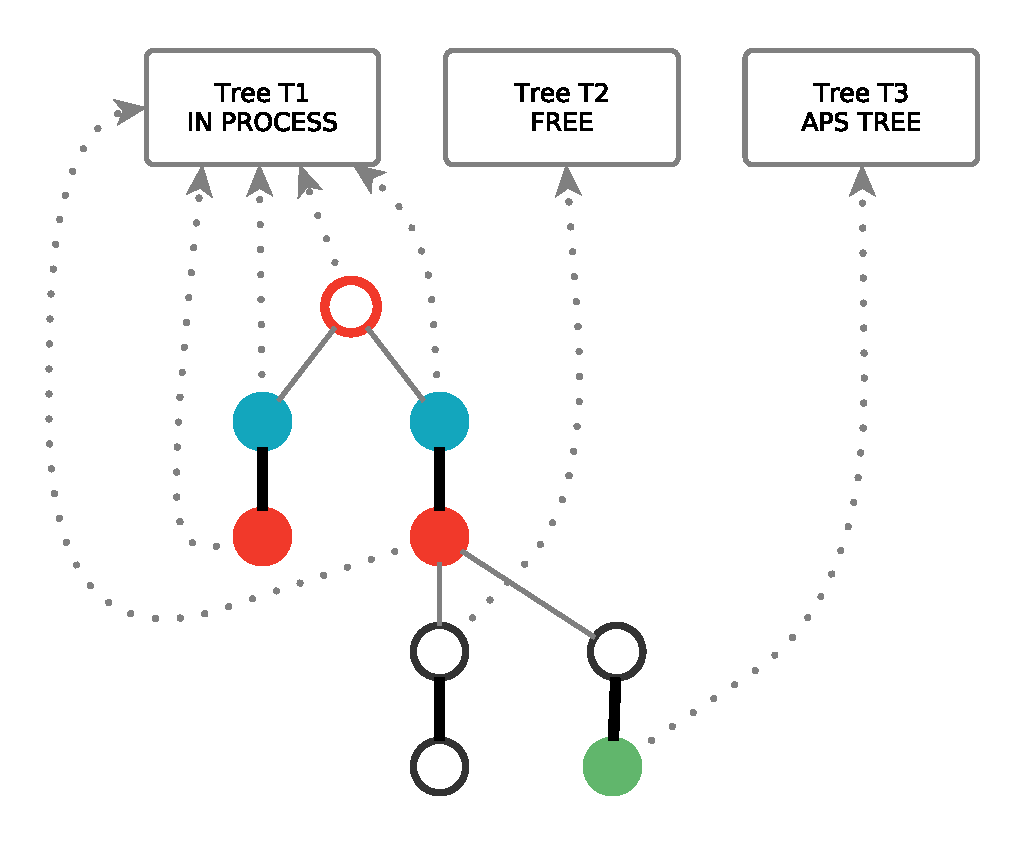
\includegraphics[scale=0.5]{img/implementation.eps}
  \caption{Datové struktury uzlu a stromu.}
  \label{imgStructure}
\end{figure}

\subsection{Popis implementace}

Algoritmus jsme implementovaly v jazyce \texttt{C}.

Datová struktura \texttt{TGraph} reprezentuje bipartitní neorientovaný graf. Obsahuje počet uzlů \texttt{n}, počet hran \texttt{m}, pole uzlů \texttt{nodes} a seznam stromů \texttt{trees}. Uzly jsou reprezentované strukturou \texttt{TNode} s položkami: pořadové číslo uzlu \texttt{id}, seznam hran \texttt{edges}, ukazatel na vstupní hranu \texttt{entry} a ukazatel na strom \texttt{tree}. Pokud uzel patří nějakému stromu, jeho ukazatel na vstupní hranu je nastavený na hranu z předchůdce uzlu do tohoto uzlu. Hranu reprezentuje struktura \texttt{TEdge}: \texttt{M} značí, zda hrana patří do dosud nalezeného párování grafu, \texttt{node} je ukazatel na uzel, do kterého hrana vstupuje, a \texttt{reversed} je ukazatel na hranu, která je k hraně opačná. Struktura \texttt{TQueue} spolu s \texttt{TItem} reprezentují abstraktní datový typ fronta.

Graf lze inicializovat, vytvořit a zrušit funkcemi \texttt{initGraph}, \texttt{loadGraph} a \texttt{freeGraph}. Strom lze vytvořit zavoláním funkce \texttt{createTree}. Funkce \texttt{processPath} projde strom od listového uzlu ke kořenovému a upraví na cestě párování. Funkce \texttt{applyAPS} se snaží nalézt $M$-rozšiřující cestu. Pokud ji nalezne, zavolá pro ni funkci \texttt{processPath} a nastaví status stromu na \texttt{FREE}, jinak nastaví status stromu na \texttt{APSTREE}. Funkce \texttt{findMatching} prochází pole uzlů \texttt{nodes} grafu \texttt{graph} a pokud některá jeho vstupní hrana není v dosud nalezeném párování, vytvoří se strom s nalezeným uzlem jako kořenem a zavolá se funkce \texttt{applyAPS}. Funkce \texttt{main} zkontroluje vstupní paramentry, ze vstupního souboru vytvoří graf a zavolá pro něj funkci \texttt{findMatching}.

\subsection{Spuštění aplikace}

Naše implementace se nachází ve složce \texttt{sequence} v souboru \texttt{matching.c}. Program lze přeložit příkazem \texttt{make} a spustit příkazem \texttt{./matching file}, kde \texttt{file} je název vstupního souboru ve formátu popsaném v kapitole \ref{secGenerating}.

%%%%%%%%%%%%%%%%%%%%%%%%%%%%%%%%%%%%%%%%%%%%%%%%%%%%%%%%%%%%%%%%%%%%%%%%%
\section{Paralelní varianta algoritmu}

\subsection{Analýza problému}

V popisu Egerváryho algoritmu si lze všimnout, že se vždy pracuje pouze s vytvářeným stromem a jeho nejbližším okolím. Pokud je nalezena $M$-rozšiřující cesta, dochází ke změnám na hranách, které patří do tohoto stromu, pokud je nalezen APS strom, přebarví se pouze uzly tohoto stromu.

Jako přirozený způsob paralelizace Egerváryho algoritmu se nabízí zpracovávání grafu více procesy tak, že každý proces bude vytvářet vlastní strom. Pokud bychom zaručily, že takové stromy budou vždy navzájem disjuktní, s ohledem na předcházející paragraf by paralelní zpracování nijak neovlivnilo fungování Egerváryho algoritmu. Na víceprocesorových počítačích by se však výpočet urychlil.

Disjuktnost stromů ale zaručit nemůžeme, proto je třeba najít způsob, jak se vypořádat s konflikty mezi stromy. Obecná situace je taková, že proces $1$ buduje strom $T_1$, proces $2$ buduje strom $T_2$ a proces $1$ bude chtít k uzlu $v_1$ svého stromu $T_1$ připojit uzel $v_2$ stromu $T_2$. Podle barev uzlů $v_1$ a $v_2$ rozlišujeme následující typy konfliktů.

Konflikt typu B-B je konflikt mezi modrým uzlem $v_1$ a modrým uzlem $v_2$. Příklad takového konfliktu je na obrázku \ref{imgXX}. Na obrázku si můžeme všimnout toho, že v takovém případě existuje $M$-rozšiřující cesta z kořene stromu $T_1$ do kořene stromu $T_2$. Nalezení cesty je žádoucí, proto pokud dojde k takovému konfliktu, lze zastavit růst obou stromů, upravit párování na hranách nalezené cesty a uzly ve stromech přebarvit na bílo, aby byly k dispozici dalším stromům. Konflikt typu R-R pro červené uzly $v_1$, $v_2$ je analogický konfliktu B-B (viz. \ref{imgXX}).

\begin{figure}[ht]
  \centering
  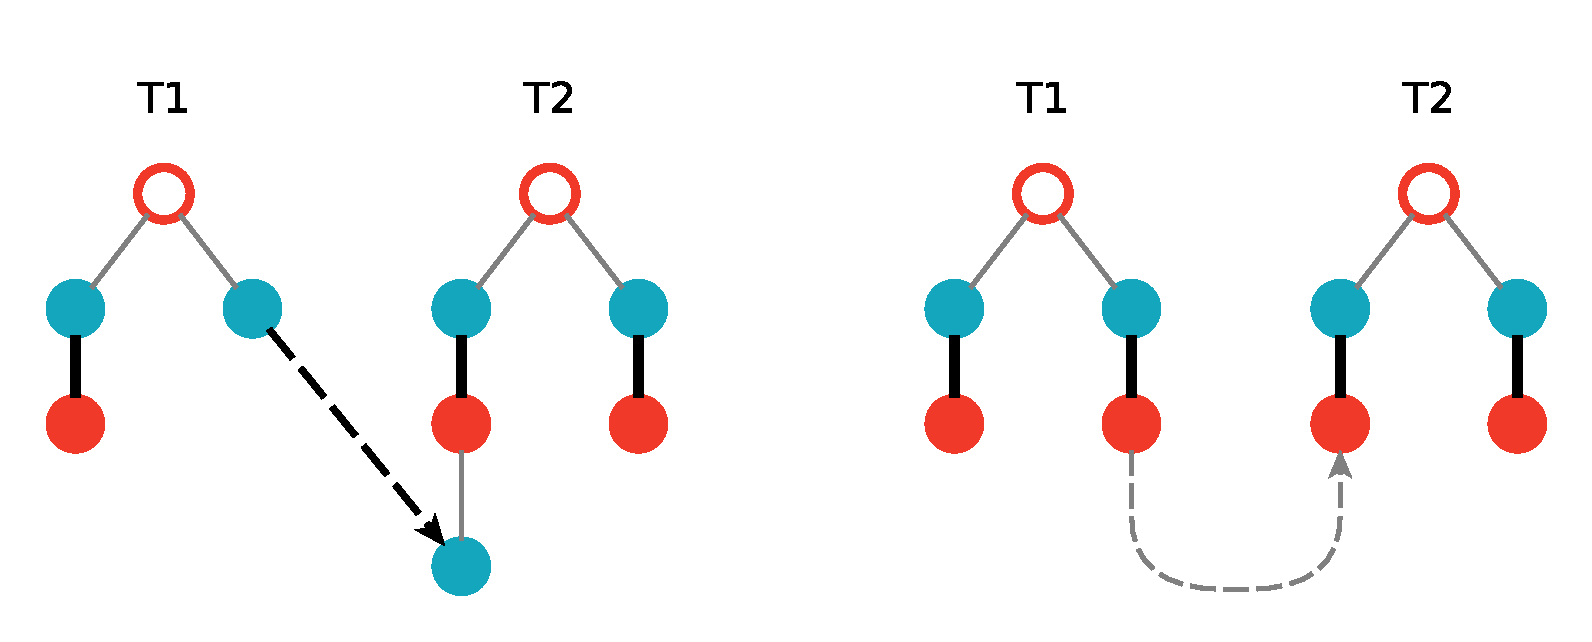
\includegraphics[scale=0.5]{img/XXconflicts.eps}
  \caption{Konflikty B-B a R-R.}
  \label{imgXX}
\end{figure}

Konflikt typu R-B je konflikt mezi červených uzlem $v_1$ a modrým uzlem $v_2$. Na obrázku \ref{imgXY} vidíme, že v tomto případě se $M$-rozšiřující cesta nevytvoří. Nabízí se několik možných řešení. Strom $T_1$ by mohl získat uzel $v_2$, pak by ale strom $T2$ nemohl pokračovat ve výpočtu a všechny jeho uzly by musely být obarveny na bílo a uvolněny. Stejně tak by mohl $T_1$ prohrát uzel $v_2$, $T_2$ by dál pokračoval ve výpočtu a $T_1$ by se ukončil. Třetí možností je ignorace konfliktní hrany. $T_2$ by dál pokračoval ve výpočtu, nijak neovlivněn tímto konfliktem. $T_1$ by taktéž pokračoval ve výpočtu, ale pokud by skončil nalezením APS stromu, tak by své uzly obarvil na bílo a vytvořený strom zahodil.

Konflikt typu B-R je konflikt mezi modrým uzlem $v_1$ a červeným uzlem $v_2$. Z obrázku \ref{imgXY} je patrné, že v takovém případě by z uzlu $v_2$ vedly dvě hrany náležící párování $M$. $M$ by potom nebylo platné párování. Párování může být dočasně neplatné jen v případě, že nějaký strom nalezl $M$-rozšiřující cestu a upravuje párování na hranách této cesty. Pokud jsou oba stromy $T_1$, $T_2$ ve fázi růstu pak párování na hranách vycházejících z uzlů těchto dvou stromů je platné a neměnné. V našem případě předpokládáme, že oba stromy rostou, proto k B-R konfliktu nemůže dojít.

\begin{figure}[ht]
  \centering
  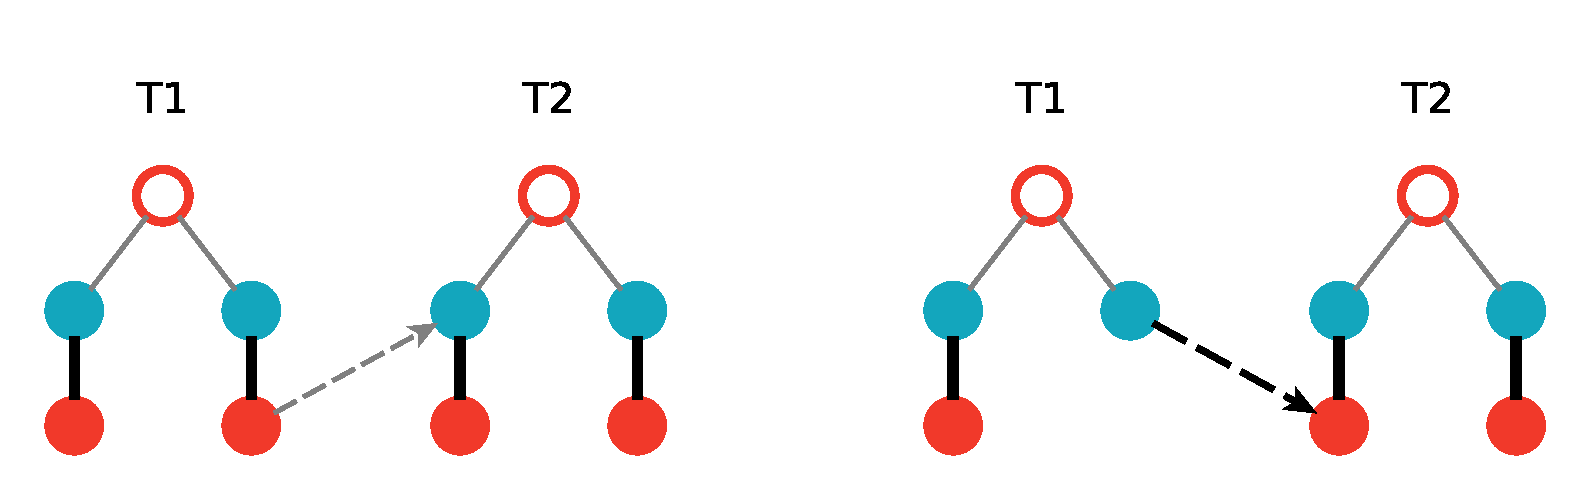
\includegraphics[scale=0.5]{img/XYconflicts.eps}
  \caption{Konflikty R-B a B-R.}
  \label{imgXY}
\end{figure}

Dále je třeba uvažovat o způsobu, jakým se budou synchronizovat procesy. Je zřejmé, že je třeba zaručit, aby s každým uzlem pracoval v jeden okamžik nejvýše jeden proces. Potom bude třeba sychnronizovat přístup ke stromům uzlů. Pokud bychom se inspirovaly návrhem sekvenčního algoritmu, pak informaci o stavu stromu nese pouze strom. Pak při každém přístupu k uzlu je potřeba nejprve zamknout příslušný strom a pak teprve uzel. Pokud očekáváme konflikt, je třeba zamknout oba stromy a konfliktní uzly. Druhou možností je propagovat informaci o stavu stromu do jeho uzlů. Pro přístup k uzlu by pak stačilo zamknutí uzlu.

\subsection{Diskuze k návrhu řešení}

Naše výsledné řešení vyplynulo z několika dalších řešení, která jsme implementovaly a testovaly. 

Konflikt typu R-B jsme původně řešily tak, že proces $1$ vyhrál uzel stromu procesu $2$, pokud jeho strom $T_1$ obsahoval více uzlů než strom $T_2$. Jinak proces $1$ prohrál a byl nucen uvolnit svůj strom. V obou případech došlo k zahození jednoho z konfliktních stromů. Vzhledem k tomu, že další dva typy konfliktů R-R a B-B výpočet urychlují, myslely jsme si, že zpomalení výpočtu konfliktem R-B se ve výsledku neprojeví. Ukázalo se, že to není pravda. K zahazování stromů docházelo neustále a počet vytvořených stromů rostl vzhledem k velikosti vstupního grafu polynomiálně. To značně zpomalovalo výpočet. Efektivnějším řešením konfliktu se ukázala být ignorace konfliktní hrany. Počet vytvořených stromů byl pak lineární a většina $M$-rozšiřujících cest byla nalezena R-R a B-B konflikty.

Synchronizaci procesů jsme zkusily řešit zamykáním stromů. Algoritmus byl tedy velmi podobný sekvenčnímu řešení. Uzly se odkazovaly na stromy a stromy obsahovaly informaci o svém stavu. Rostoucí strom byl ve stavu \texttt{INPROCESS}. Vyvoření APS stromu bylo možné nastavením stavu na \texttt{APSTREE}. Uvolnění stromu proběhlo upravením stavu na \texttt{FREE}. Úprava stavu tak sice byla možná v konstatním čase, ale kdykoliv chtěl proces přidat ke svému stromu nový uzel, musel zamknout svůj strom i strom toho uzlu. Stromy se tak staly úzkým hrdlem programu. To se projevilo zejména tak, že s vyšším počtem dostupných procesorů se časová efektivita programu nezlepšovala.

Řešením tohoto problému byla propagace stavu stromu ze stromu do uzlů. Stav stromu pak bylo možné vyčíst z barvy jeho uzlu. Bílý uzel nepatřil žádnému stromu, zelený uzel patřil APS stromu, modrý a červený uzel patřil zpracovávenému stromu. Toto řešení je výhodné v tom, že pokud chce proces přidat ke svému stromu nový uzel, vyčte z barvy tohoto uzlu, jestli má komunikovat i s jeho stromem, nebo ne. Nevýhodou je časová složitost přebarvení všech uzlů stromu. Důležité však je, že se takto zjednodušila synchronizace, což umožnilo více využívat dostupné procesory.

\subsection{Návrh řešení}

Na začátku jsou všechny uzly obarveny na bílo a vloženy do fronty kořenových uzlů. Pokud je kořenová fronta prázdná, proces $i$ se ukončí, jinak z fronty vyzvedne uzel $u$. Pokud je uzel $u$ bilý, proces jej přidá do svého stromu $T_i$ jako kořen a obarví jej na červeno. Proces $i$ začne hledat $M$-rozšiřující cestu. Postupně připojuje k uzlům $v_i$ uzly $v_j$. 

Pokud se pokusí přidat bílý uzel $v_j$, proces uzel obarví na červenou nebo modrou a přivlastní si jej. Pokud se pokusí přidat zelený uzel $v_j$, pak jej ignoruje, neboť uzel patří do APS stromu. Pokud se pokusí přidat červený nebo modrý uzel $v_j$, došlo ke konfliktu. 

\begin{figure}[ht]
  \centering
  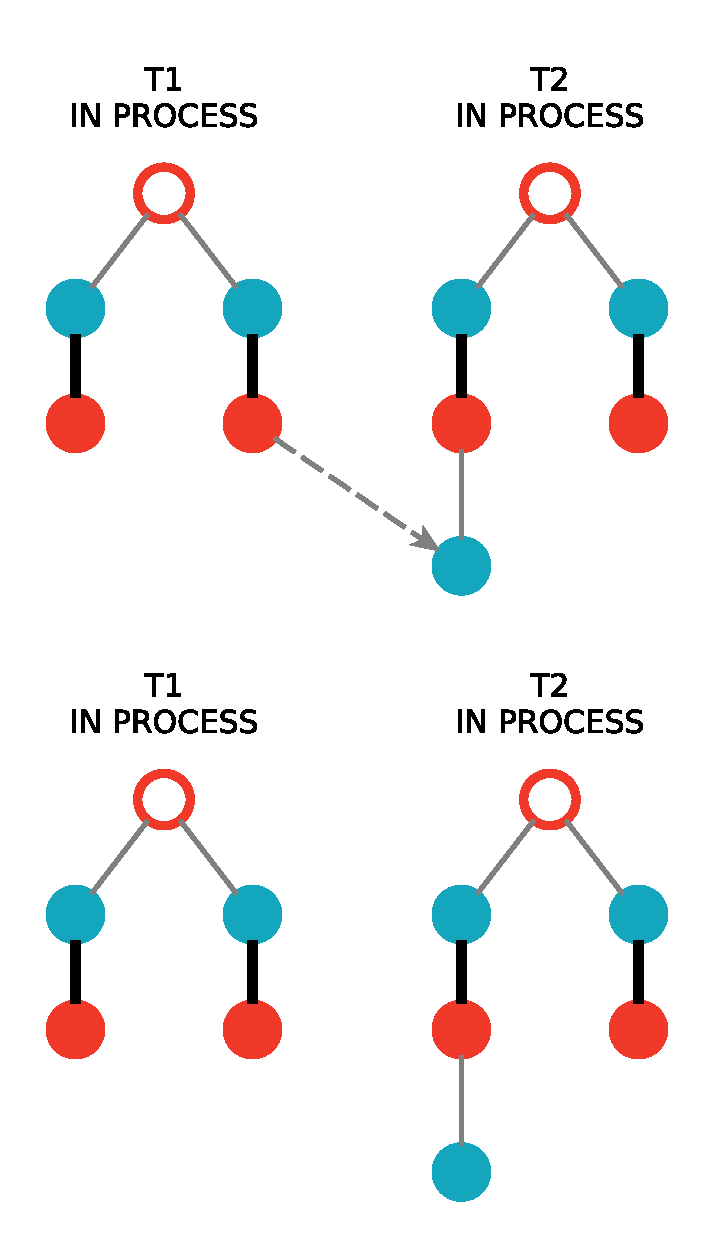
\includegraphics[scale=0.5]{img/inconflict.eps}
  \caption{Řešení R-B konflitu.}
  \label{imgConflict}
\end{figure}

V případě R-B konfliktu proces uzel ignoruje (viz. obrázek \ref{imgConflict}). V případě R-R a B-B konfliktu proces přistoupí ke stromu uzlu. Jestliže je strom $T_j$ ve stavu \texttt{HASPATH}, pak proces uzel ignoruje. Pokud je strom ve stavu \texttt{INPROCESS}, je nalezena $M$-rozšiřující cesta (viz. obrázek \ref{imgHasPath}). Pak proces změní stav stromu $T_j$ na \texttt{HASPATH} a nastaví stromu ukazatel na konec cesty. Následně změní stav svého stromu $T_i$ na \texttt{HASPATH} a nastaví mu ukazatel na konec cesty. Nakonec upraví párování hrany z $v_i$ do $v_j$.

\begin{figure}[ht]
  \centering
  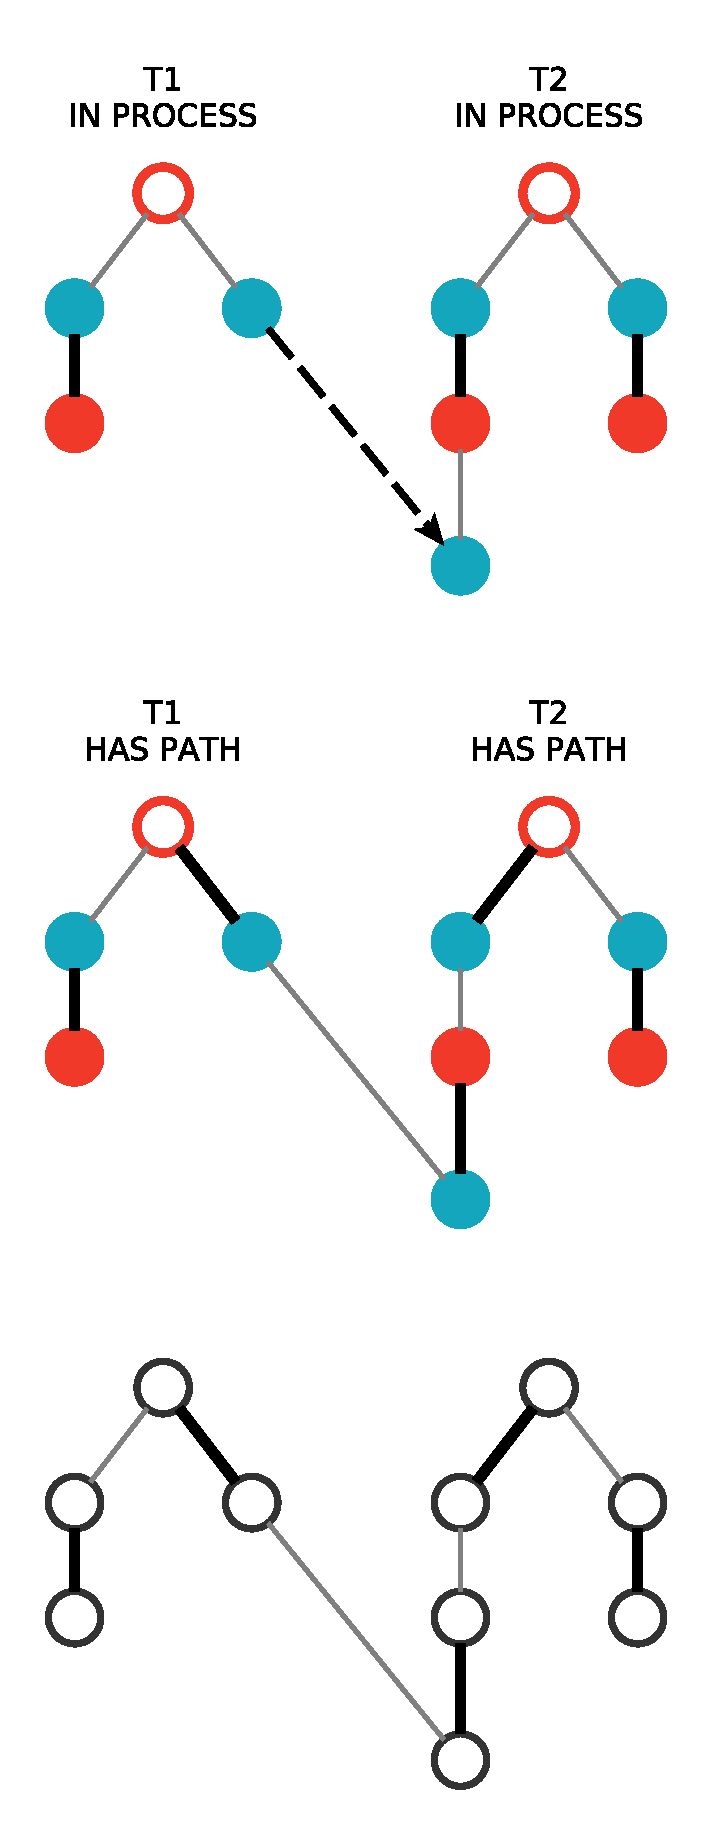
\includegraphics[scale=0.5]{img/haspath.eps}
  \caption{Řešení R-R a B-B konfliktu.}
  \label{imgHasPath}
\end{figure}

Pokud proces $i$ nalezne cestu, nastaví stav stromu $T_i$ na \texttt{HASPATH}. Pokud proces $i$ zjistí, že jeho strom je ve stavu \texttt{HASPATH}, pak upraví párování na nalezené cestě, změní jeho stav na \texttt{FREE} a obarví všechny jeho uzly na bílo. Pokud proces $i$ skončí hledání $M$-rozšiřující cesty nalezením APS stromu a strom $T_i$ nevyvolal žádné R-B konflikty, pak proces nastaví stav stromu na \texttt{APSTREE} a obarví všechny jeho uzly na zeleno. Jestliže strom $T_i$ nějaký R-B konflikt vyvolal, pak proces nastaví jeho stav na \texttt{FREE} a obarví všechny jeho uzly na bílo. Nakonec si proces $i$ vyvedne z fronty kořenových uzlů nový uzel a celý proces se opakuje.

\subsection{Popis implementace}

Algoritmus jsme implementovaly v jazyce \texttt{C} s využitím knihovny \texttt{pthread}. 

Datové struktury \texttt{TList} a \texttt{TQueue} reprezentují abstraktní datové typy seznam a fronta nad prvky typu ukazatel na \texttt{void}. \texttt{TGraph}, \texttt{TTree}, \texttt{TNode} a \texttt{TEdge} jsou v podstatě stejné jako u sekvenční varianty. Liší se zejména přítomností mutexů, které zajišťují exkluzivní přístup ke strukturám (z výjimkou \texttt{TEdge}). \texttt{TTree} si navíc uchovává pořadové číslo stromu \texttt{id}, pořadové číslo \texttt{owner} procesu, který ho vlastní, ukazatel \texttt{pathEnd} na konec cesty a seznam uzlů \texttt{nodes}, které jsou ve stromu. Vlákno je reprezentováno datovým typem \texttt{TThread}, mutex typem \texttt{TMutex}. Datová struktura \texttt{TThreadData} zapouzdřuje vstupní data procesů.

Graf lze inicializovat, vytvořit a zrušit funkcemi \texttt{initGraph}, \texttt{loadGraph} a \texttt{freeGraph}. Zamykání uzlů a stromů umožňují funkce \texttt{lockNode}, \texttt{unlockNode}, \texttt{lockTree}, \texttt{unlockTree}, \texttt{lockNodes} a \texttt{lockTrees}, přičemž funkce \texttt{lockNodes} a \texttt{lockTrees} zamykají dvojice uzlů nebo stromů v pořadí určeném jejich \texttt{id}. Strom lze vytvořit a zrušit zavoláním funkce \texttt{createTree} a \texttt{freeTree}. Funkce \texttt{colourNodes} obarví všechny uzly stromu na požadovanou barvu, \texttt{processPath} projde stromem od listového uzlu ke kořeni a změní na hranách cesty párování.

Funkce \texttt{addNodeToTree} se snaží k uzlu \texttt{nodeA} stromu \texttt{treeA} přidat uzel \texttt{nodeB} přes hranu \texttt{AB} s očekávanou příslušností k párování \texttt{M}. Funkce vrací hodnotu z výčtu: \texttt{OK}, \texttt{ABORT}, \texttt{IGNORE}, \texttt{CONFLICT} nebo \texttt{PATH}. 

Funkce \texttt{applyAPS} se pomocí stromu \texttt{tree} snažít nalézt $M$-rozšiřující cestu. Pokud nalezne cestu, zavolá na ni \texttt{processPath}, funkcí \texttt{colourNodes} obarví uzly stromu na bílo a vrátí \texttt{OK}. Pokud nalezne APS strom, obarví uzly na zeleno a vrátí \texttt{OK}. Jinak obarví uzly na bílo a vrátí \texttt{ABORT}.

Funkce \texttt{findMatching} zpracovává frontu kořenových uzlů. Pokud fronta není prázdná, vybere se uzel, který je bílý a žádná jeho hrana není v párování. Vytvoří se strom, kde vybraný uzel bude jeho kořenovým uzlem, a zavolá se funkce \texttt{applyAPS}. Pokud funkce vrátí \texttt{ABORT}, uzel se vrátí zpátky do fronty. Funkce \texttt{findMatchingParallel} vytváří a spouští vlákna nad funkcí \texttt{findMatching} s daty typu \texttt{TThreadData}. Funkce \texttt{main} kontroluje vstupní parametry, vytváří ze vstupního souboru graf a volá pro něj funkci \texttt{findMatchingParallel}.

\subsection{Spuštění aplikace}

Výsledný program \texttt{matching.c} je umístěný v adresáři \texttt{parallel}. Lze jej přeložit příkazem \texttt{make} a spustit příkazem \texttt{./matching file n}, kde \texttt{file} je název vstupního souboru a \texttt{n} je počet vláken. Očekáváný formát vstupního souboru popisujeme v kapitole \ref{secGenerating}.

%%%%%%%%%%%%%%%%%%%%%%%%%%%%%%%%%%%%%%%%%%%%%%%%%%%%%%%%%%%%%%%%%%%%%%%%%
\section{Experimenty}

\subsection{Generování vstupních souborů} \label{secGenerating}

Pro vygenerování vstupních souborů jsme v jazyce \texttt{python 2.7} s použitím knihovny \texttt{python-igraph 0.7} napsaly skript \texttt{generator.py}. 
Skript generuje bipartitní neorientované grafy $G=(X,Y,E)$ a ukladá je do souborů \texttt{graph\_x\_y\_p\_m}, kde $x$ je počet uzlů v množině $X$, $y$ je počet uzlů v množině $Y$, $p$ je procentuální vyjádření počtu hran množiny $E$ a $m$ je počet hran v maximálním párování. Pak soubor obsahuje počet uzlů množiny $X \cup Y$, počet hran množiny $E$ a výčet všech dvojic uzlů, mezi kterými existuje v $E$ hrana, přičemž každá hrana je reprezentovaná právě jednou.

Skript je umístěný ve složce \texttt{graph}. Příkazem \texttt{python2.7 generator.py} se podle parametrů nastavených ve scriptu vygeneruje soubor s náhodným grafem. Příkaz \texttt{python2.7 generator.py test} vygeneruje všechny testovací soubory pro naše experimenty. Knihovna \texttt{python-igraph} na školním serveru \texttt{merlin} není dostupná, proto v archivu odevzdáváme část testovacích souborů.



%%%%%%%%%%%%%%%%%%%%%%%%%%%%%%%%%%%%%%%%%%%%%%%%%%%%%%%%%%%%%%%%%%%%%%%%%
\section{Závěr}

%------------------------------------------------------------------------
\begin{thebibliography}{1}
  
  \bibitem{bondy:2008} BONDY, J. A. a U. S. R. MURTY. \emph{Graph theory}. New York: Springer, 2008, xii, 651 s. ISBN 978-1-84628-969-9. 
  
  \bibitem{igraph:2003} \emph{Python-igraph} [online]. \copyright 2003-2013 [cit. 2014-12-13]. Dostupné z: http://igraph.org/python/ 

\end{thebibliography}


%------------------------------------------------------------------------
\end{document}

% end of file
